% This file was created by matplotlib2tikz v0.7.4.
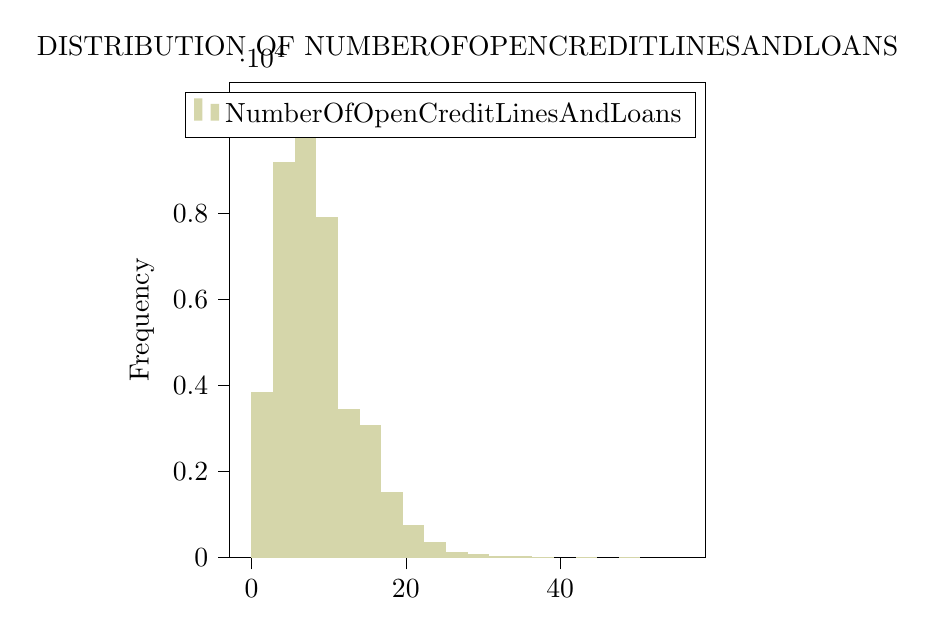
\begin{tikzpicture}

\definecolor{color0}{rgb}{0.835294117647059,0.83921568627451,0.666666666666667}

\begin{axis}[
height=3in,
tick align=outside,
tick pos=left,
title={\printsubsection{\MakeUppercase{Distribution of NumberOfOpenCreditLinesAndLoans}}\\},
width=3in,
x grid style={white!69.01960784313725!black},
xmin=-2.8, xmax=58.8,
xtick style={color=black},
y grid style={white!69.01960784313725!black},
ylabel={Frequency},
ymin=0, ymax=11054.4,
ytick style={color=black}
]
\draw[fill=color0,draw opacity=0] (axis cs:0,0) rectangle (axis cs:2.8,3858);
\addlegendimage{ybar,ybar legend,fill=color0,draw opacity=0};
\addlegendentry{NumberOfOpenCreditLinesAndLoans}

\draw[fill=color0,draw opacity=0] (axis cs:2.8,0) rectangle (axis cs:5.6,9205);
\draw[fill=color0,draw opacity=0] (axis cs:5.6,0) rectangle (axis cs:8.4,10528);
\draw[fill=color0,draw opacity=0] (axis cs:8.4,0) rectangle (axis cs:11.2,7920);
\draw[fill=color0,draw opacity=0] (axis cs:11.2,0) rectangle (axis cs:14,3465);
\draw[fill=color0,draw opacity=0] (axis cs:14,0) rectangle (axis cs:16.8,3076);
\draw[fill=color0,draw opacity=0] (axis cs:16.8,0) rectangle (axis cs:19.6,1535);
\draw[fill=color0,draw opacity=0] (axis cs:19.6,0) rectangle (axis cs:22.4,748);
\draw[fill=color0,draw opacity=0] (axis cs:22.4,0) rectangle (axis cs:25.2,359);
\draw[fill=color0,draw opacity=0] (axis cs:25.2,0) rectangle (axis cs:28,124);
\draw[fill=color0,draw opacity=0] (axis cs:28,0) rectangle (axis cs:30.8,92);
\draw[fill=color0,draw opacity=0] (axis cs:30.8,0) rectangle (axis cs:33.6,49);
\draw[fill=color0,draw opacity=0] (axis cs:33.6,0) rectangle (axis cs:36.4,28);
\draw[fill=color0,draw opacity=0] (axis cs:36.4,0) rectangle (axis cs:39.2,10);
\draw[fill=color0,draw opacity=0] (axis cs:39.2,0) rectangle (axis cs:42,2);
\draw[fill=color0,draw opacity=0] (axis cs:42,0) rectangle (axis cs:44.8,6);
\draw[fill=color0,draw opacity=0] (axis cs:44.8,0) rectangle (axis cs:47.6,3);
\draw[fill=color0,draw opacity=0] (axis cs:47.6,0) rectangle (axis cs:50.4,4);
\draw[fill=color0,draw opacity=0] (axis cs:50.4,0) rectangle (axis cs:53.2,3);
\draw[fill=color0,draw opacity=0] (axis cs:53.2,0) rectangle (axis cs:56,1);
\end{axis}

\end{tikzpicture}